\subsection{Ayasofya Medresesi}
\indent\indent Ayasofya Camii etrafında Türkler’in inşa ettiği külliye parçalarından biri olarak yapılmıştır. İstanbul’un fethinin hemen arkasından ilk ihtiyacı karşılamak üzere Ayasofya’nın yanındaki papaz odaları medrese haline getirilmişti. Bu odaların Ayasofya’ya komşu olduğu bilinen patrikhânenin bir kısmı olduğuna da ihtimal verilebilir. Fâtih Sultan Mehmed vakfiyelerinden öğrenildiğine göre esas Ayasofya Medresesi bizzat Fâtih’in vakfı olarak cami yanına inşa edilmiştir. Fakat Fâtih Camii ve manzumesi yapıldıktan sonra bir süre boş kalmış, II. Bayezid devrinde tekrar açılmıştır. Müderrisleri arasında XV. yüzyılın ünlü bilginlerinden Molla Hüsrev ile Fâtih Külliyesi yapılıncaya kadar Ali Kuşçu da bulunmuştur. Medresenin kapısı yanında Akşemseddin’in bir halvethânesinin mevcut olduğunu yine Hüseyin Ayvansarâyî bildirmektedir.\newline
\indent 10 Cemâziyelevvel 1005 (30 Aralık 1596) tarihli bir masraf defterinden öğrenildiğine göre, bir süre önce yıktırılmış olan Ayasofya Medresesi bu tarihte tamir ve ihya edilmiştir. Medrese herhalde birkaç tamir veya değişiklik daha gördükten sonra, Sultan Abdülmecid tarafından 1846-1849 yılları arasında İsviçreli mimar Gaspare Fossati’ye yaptırılan büyük tamir sırasında, temelden itibaren tamamen yeniden yapılmıştir.\newline
\indent Ayasofya Medresesi 1924 yılına kadar kullanıldıktan sonra İstanbul Belediyesi’nce öksüzler yurdu haline getirilmiş, 1934’te Ayasofya Camii’nin Vakıflar İdaresi’nden alınarak Müzeler Genel Müdürlüğü’ne devredilmesinden sonra kısa bir süre daha yurt olarak kullanılmış, 1935 yılında boşaltılmıştır. Bu tarihte Ayasofya’nın etrafını açmak gayesi ve mevcut medrese binasının “eski eser” özelliğinde olmadığı gerekçesiyle Müzeler İdaresi tarafından tamamen yıktırılmıştır. 1985-1986 yıllarında medrese arsasındaki toprak ve moloz yığını kaldırılmış ve binanın temelleri bulunmuştur.\cite{dia_9}\newline
\begin{figure}[H]
    \centering
    \subfigure[Medresenin Bahçesi]{
        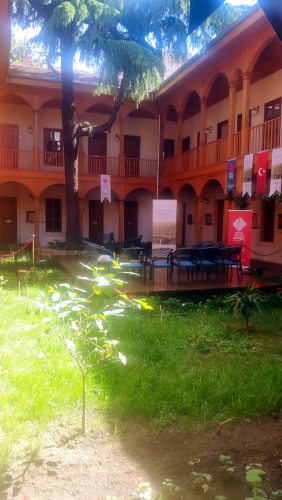
\includegraphics[height=0.45\textheight]{assets/medrese.jpg}
    }
    \subfigure[Eski Medresenin Kalıntıları]{
        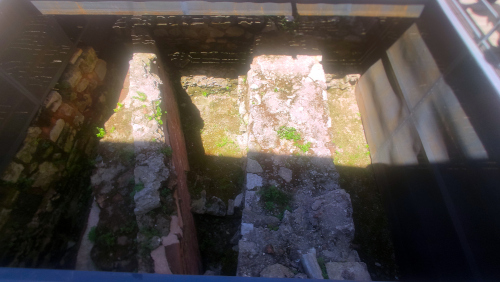
\includegraphics[width=0.95\textwidth]{assets/medrese_ruins.jpg}
    }
    \caption{Ayasofya Medresesi}
\end{figure}

